% !TeX program = xelatex
\documentclass[UTF8,11pt,a4paper,fontset=none]{ctexart}
\usepackage[margin=23mm,headheight=16pt,footskip=13mm]{geometry}
\usepackage{fontspec}
\setmainfont{Noto Sans}
\setsansfont{Noto Sans}
\setmonofont[Scale=0.85]{DejaVu Sans Mono}
\setCJKmainfont{Noto Sans CJK TC}
\setCJKsansfont{Noto Sans CJK TC}
\setCJKmonofont{Noto Sans Mono CJK TC}
\xeCJKDeclareCharClass{CJK}{"2460 -> "2473, "2190 -> "2193}
\usepackage{amsmath,graphicx,booktabs,tabularx,longtable,array,multirow}
\usepackage[table]{xcolor}
\usepackage{enumitem,fancyhdr,tcolorbox,caption,float}
\usepackage{hyperref,xurl}
\definecolor{navy}{HTML}{16324F}
\definecolor{teal}{HTML}{087F8C}
\definecolor{light}{HTML}{EFF5F8}
\definecolor{muted}{HTML}{536578}
\definecolor{amber}{HTML}{8F5310}
\hypersetup{unicode=true,colorlinks=true,linkcolor=navy,urlcolor=teal,citecolor=teal,
  pdftitle={Saccade v1：偵測模型是怎麼訓練出來的},
  pdfauthor={Saccade v1 專案},pdfsubject={資料、四個訓練階段、選模、逐步改進與 TensorRT 匯出}}
\urlstyle{same}
\renewcommand{\contentsname}{目錄}
\renewcommand{\refname}{證據與參考文件}
\ctexset{section={format=\Large\bfseries\sffamily\color{navy}},
  subsection={format=\large\bfseries\sffamily\color{navy}},
  subsubsection={format=\normalsize\bfseries\sffamily}}
\clubpenalty=10000
\widowpenalty=10000
\setlength{\parindent}{2em}
\setlength{\parskip}{0.35em}
\linespread{1.18}
\setlength{\emergencystretch}{1.5em}
\setlength{\tabcolsep}{5pt}
\renewcommand{\arraystretch}{1.30}
\newcolumntype{Y}{>{\raggedright\arraybackslash}X}
\newcolumntype{P}[1]{>{\raggedright\arraybackslash}p{#1}}
\setlist[itemize]{leftmargin=1.7em,itemsep=0.25em,topsep=0.35em}
\setlist[enumerate]{leftmargin=1.9em,itemsep=0.3em,topsep=0.35em}
\captionsetup{font=small,labelfont={bf,color=navy},skip=8pt}
\pagestyle{fancy}\fancyhf{}
\fancyhead[L]{\small\sffamily\color{muted}Saccade v1｜模型訓練}
\fancyhead[R]{\small\sffamily\color{muted}圖解版 v1.0}
\fancyfoot[L]{\scriptsize\color{muted}2026-11-13｜部署權重 Full25 e10・engine 8292cc23}
\fancyfoot[R]{\small\thepage}
\renewcommand{\headrulewidth}{0.4pt}
\newtcolorbox{finding}[1][]{colback=light,colframe=teal,boxrule=0.7pt,
  arc=1mm,left=3mm,right=3mm,top=2mm,bottom=2mm,#1}
\newcommand{\code}[1]{\texttt{\detokenize{#1}}}
\DeclareUrlCommand\sha{\def\UrlFont{\ttfamily\small}}
\DeclareUrlCommand\cmd{\def\UrlFont{\ttfamily}}
\begin{document}
\noindent{\small\sffamily\color{teal}SACCADE v1・訓練筆記}\par
\vspace{2mm}
\noindent{\LARGE\bfseries\sffamily\color{navy}偵測模型是怎麼\\訓練出來的}\par
\vspace{3mm}
\noindent{\large\color{muted}從官方 YOLO26m 到部署中的 HR Mamba：資料、四個階段、選模與匯出。}\par
\vspace{1mm}

\section{先看整條訓練鏈}
追蹤流程每一幀都要先回答「畫面裡哪裡有人」。偵測模型分成兩半：\textbf{YOLO26m 的 backbone／neck} 把 1280×768 的影像變成三個尺度的特徵（P3／P4／P5）；\textbf{Mamba spatial head} 沿畫面四個方向掃描這些特徵，輸出每個位置「是不是人」與「框多大」。

兩半不是一次訓練出來的：先把官方 YOLO26m 整個微調成會找 MOT 行人的 \textbf{Teacher}；再凍結 Teacher，讓新的 Mamba head 先\textbf{模仿}它的輸出，最後改用\textbf{標註答案}修正。

\begin{figure}[H]
\centering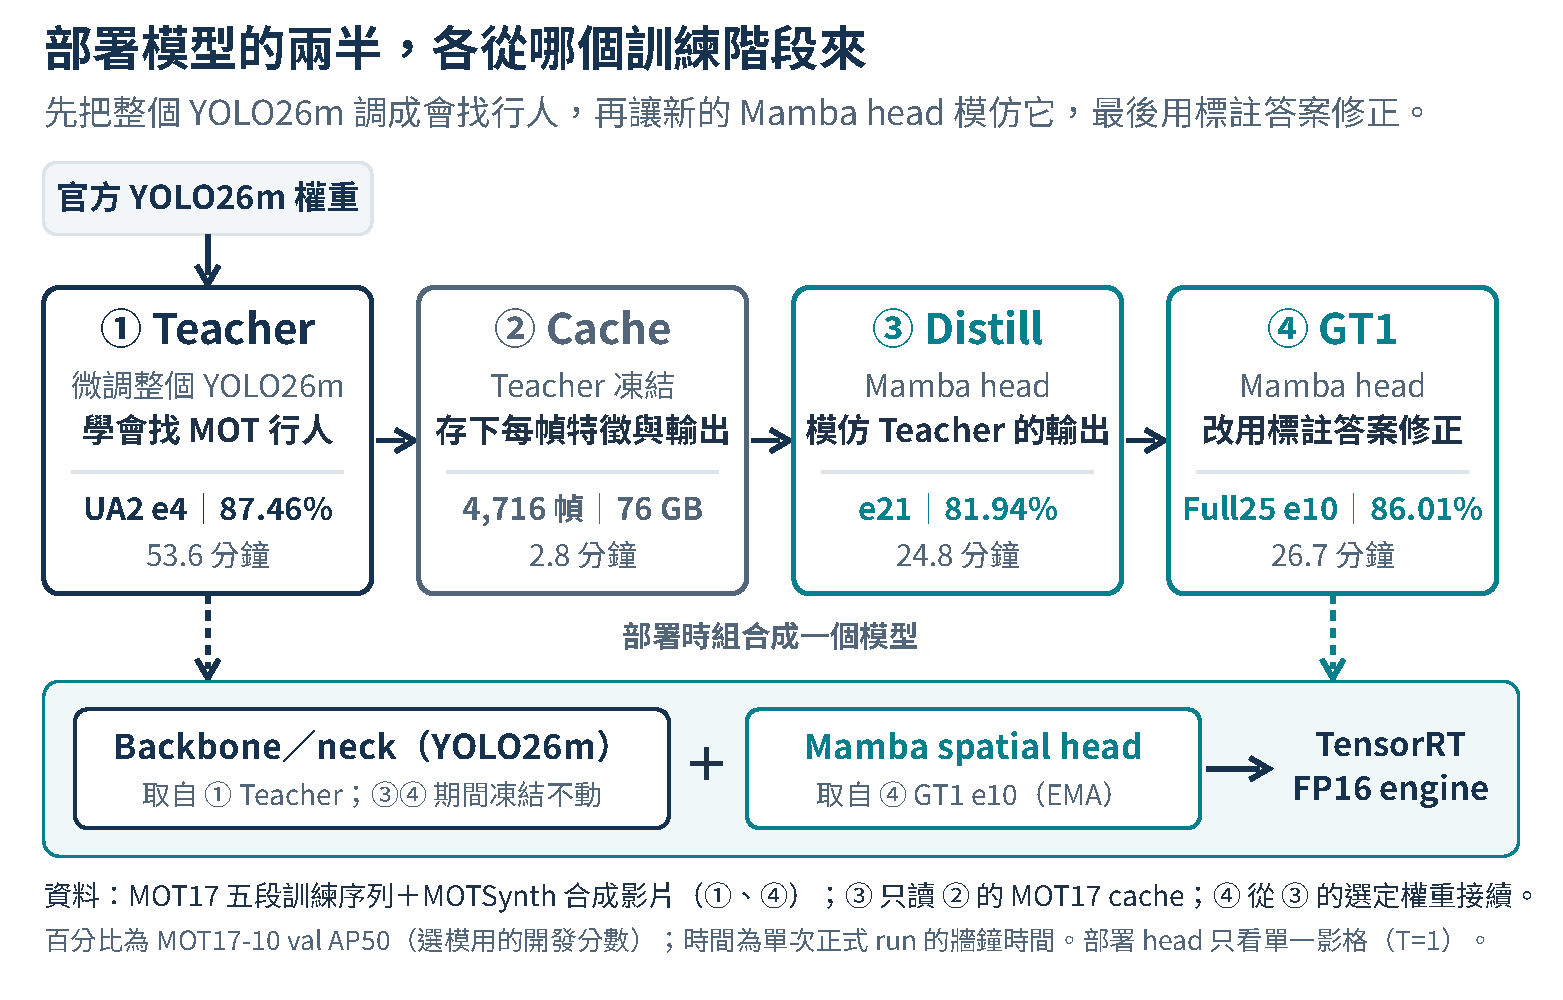
\includegraphics[width=0.84\textwidth]{assets/train-chain.pdf}
\caption{部署這一版的四個訓練階段。百分比是選模用的 MOT17-10 AP50；時間為單張 RTX 5070 Ti Laptop（12 GiB）上的實測。}
\end{figure}

\begin{finding}
\textbf{三件事先記住}\par
① 部署權重＝UA2 Teacher 的 backbone＋Full25 GT1 第 10 輪的 head，四個階段合計約 108 分鐘。\par
② 所有「選哪一版」的決定只看 MOT17-10；MOT17-02 在選定後才打開一次。\par
③ 這條配方是 10／30 到 11／03 之間、十多次正式訓練比較出來的（第 5 節）；分數多是單一 seed、單一驗證序列。
\end{finding}

\clearpage
\section{資料：誰拿來訓練、誰拿來選、誰留到最後}
\begin{figure}[H]
\centering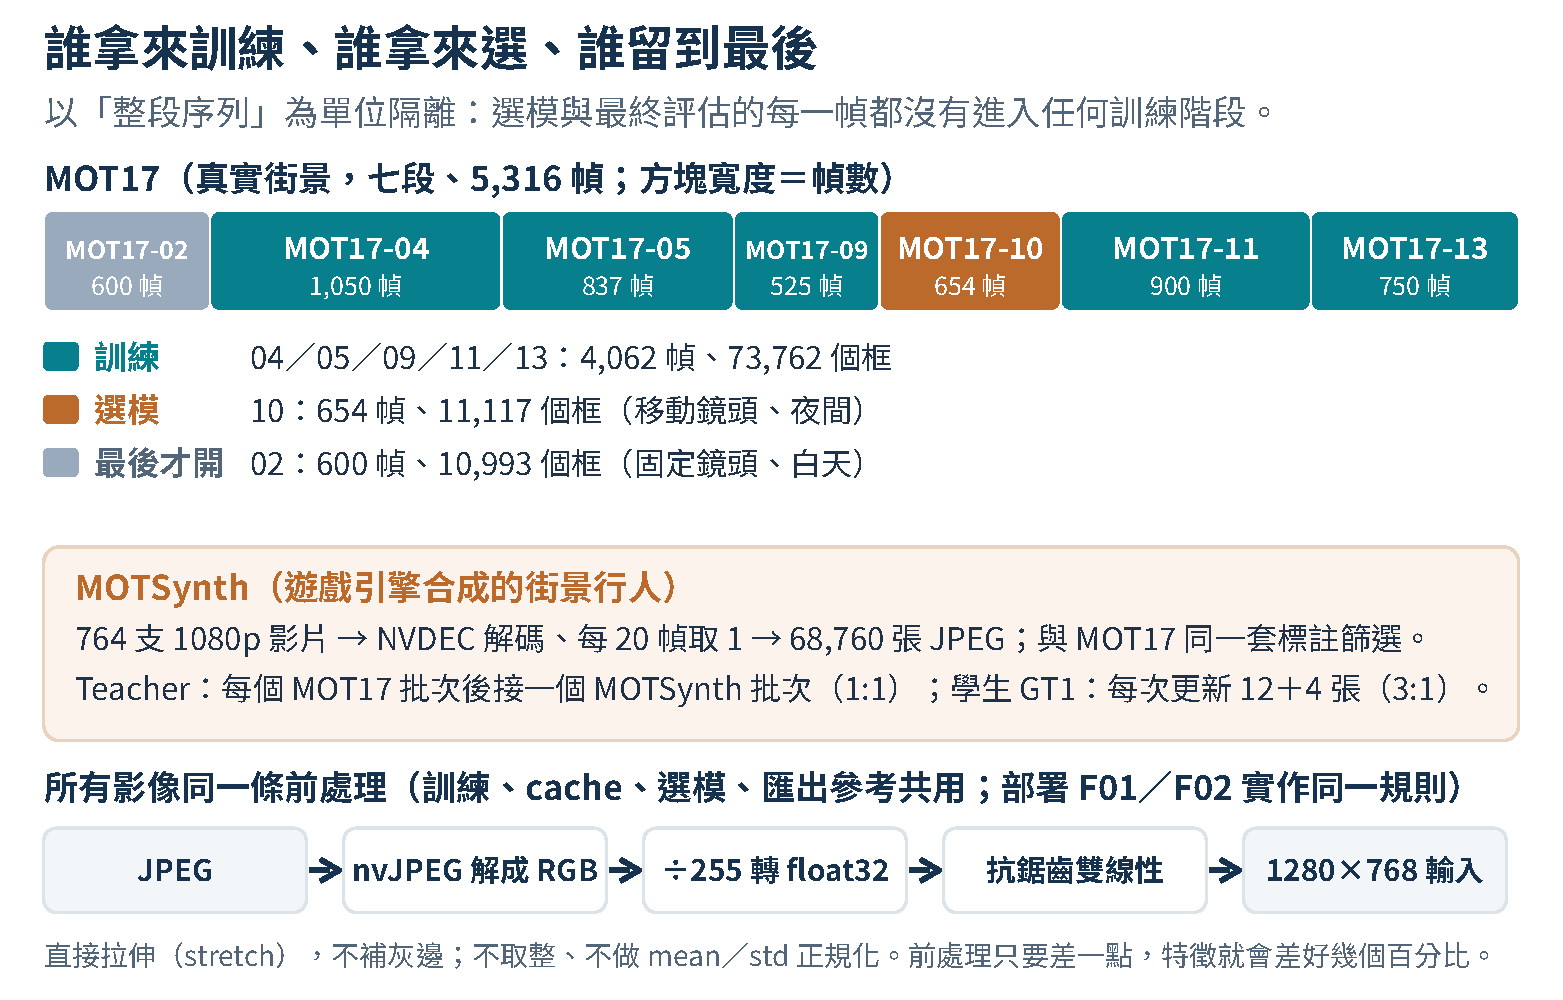
\includegraphics[width=\textwidth]{assets/train-data.pdf}
\caption{MOT17 以整段序列為單位分工；MOTSynth 只作為額外訓練資料，不參與選模。}
\end{figure}

\textbf{為什麼這樣切。} 只有 02、10、13 含大量最短邊 4--8 px 的小行人。若拿別段當驗證，選模就看不到小目標，所以 10 用來選模、02 留到最後、13 留在訓練裡提供小目標。10 是移動鏡頭的夜間街景，02 是固定鏡頭的白天，兩者條件刻意不同。驗證、評估與訓練序列之間，縮圖相似度最高只有 0.587（重複判定門檻 0.95），沒有近似重複的影格。\cite{t01}

\textbf{為什麼加合成資料。} 只用五段 MOT17 時，Teacher 在第 2 輪達到高點後就開始退步；同一批權重在\textbf{訓練序列} MOT17-13 上卻持續變好（AP50 90.0→94.9），是典型的過度擬合。CrowdHuman 與 MOTSynth 都試過：MOTSynth 讓 Teacher 的選定點高 1.44 個百分點、誤檢少 350 個；CrowdHuman 幾乎沒改變選定點，兩者合用也沒有勝過只加 MOTSynth，所以只留下 MOTSynth。\cite{hrtrain}

\textbf{為什麼前處理要寫死。} 實測顯示，輸入平均只差不到 0.3 個灰階值，backbone 特徵就會差好幾個百分比：只把解碼與縮放換成另一種實作，三個尺度的特徵就差 10.5\%／17.2\%／14.0\%；用 TF32 而不是嚴格 FP32 算特徵，也差約 1\%。因此訓練、cache、驗證與匯出參考共用同一個 nvJPEG 解碼與縮放函式，cache 一律以嚴格 FP32 計算；部署端的 F01／F02 也實作同一規則。\cite{t01}

\textbf{為什麼是 1280×768。} 640×640 會把 1920 寬的畫面壓到三分之一，瘦長的行人主要被水平壓扁。1280×768 兩軸縮放比接近（0.667／0.711），像素量只有 1280² 的 60\%，而且長寬都是 128 的倍數，head 的降採樣與還原才能對齊。\cite{hrtrain}

\clearpage
\section{四個階段各學什麼}
\begin{table}[H]
\small
\begin{tabularx}{\textwidth}{@{}P{1.55cm} P{2.3cm} Y P{2.5cm}@{}}
\toprule
階段 & 誰在學 & 怎麼學 & 選定／時間 \\
\midrule
① Teacher & 整個 YOLO26m（官方權重起步） & MOT17＋MOTSynth 交替；用標註框直接學偵測。累積到每次更新 64 張、AdamW 1.19e-4、前 3 輪 warmup、權重 EMA；翻轉、亮度／對比、縮放／平移增強 & 第 4 輪（9 輪後早停）；53.6 分 \\
② Cache & 不學習 & Teacher 逐幀前向，存 P3／P4／P5 與 Teacher 自己的分類／框輸出；嚴格 FP32 計算、FP16 儲存 & 4,716 幀、76 GB；2.8 分 \\
③ Distill & Mamba head & 讀 cache，讓 head 的輸出逼近 Teacher 的輸出（均方誤差）；掃描內部參數先固定，外圍層學習 & 第 21 輪（共 30 輪）；24.8 分 \\
④ GT1 & Mamba head（由 ③ 接續） & 改用標註答案的偵測 loss；掃描內部也一起學。每次更新 12 張 MOT17＋4 張 MOTSynth；權重 EMA 0.998 & 第 10 輪（15 輪後早停）；26.7 分 \\
\bottomrule
\end{tabularx}
\caption{部署 lineage 的四個階段。完整超參數見附錄 A。}
\end{table}

\textbf{Cache 是省力步驟。} Teacher 凍結以後，同一張圖的特徵永遠一樣，所以先算一次存起來（每幀 16 MB），學生訓練時直接讀，不必每一步重跑 backbone。

\textbf{為什麼先模仿、再對答案。} 新 head 一開始什麼都不會；直接拿標註答案訓練，訊號既稀疏又難。Teacher 的輸出對每個位置都給出「像不像人」的連續分數，先模仿它，head 很快就能接近 Teacher 的水準。但 Teacher 的分數偏寬鬆，模仿來的 head 也帶著大量低信心誤檢。以用 UA2 Teacher 重訓的那一輪（UA2D）為例：Distill 選定點在 0.25 門檻有 4,395 個誤檢；接著做 GT1，同一門檻的誤檢降到 1,618，AP50 提高 3.33 個百分點。\cite{hrtrain}

\textbf{GT1 不是把小目標丟掉。} 在 0.25 門檻下，GT1 的小目標召回率比 Distill 低；但把門檻降到 0.001，兩者找得到的小目標幾乎一樣（89.7\% 對 89.5\%）。差別在於 GT1 把一部分小目標的分數壓到 0.25 以下，這是分數校準的取捨。\cite{hrtrain}

\textbf{MOTSynth 的特徵不另外存。} 學生階段若把 MOTSynth 也做成 cache，需再多約 49 GB。這一版改成訓練時由凍結的 Teacher 即時計算（同樣嚴格 FP32、同樣轉 FP16），每輪多約 40 秒；16 張影像實測與 cache 版逐位元相同。\cite{hrmixed}

\textbf{部署 head 只看單一影格。} GT1 每次更新的 16 張影像分成四份，各自獨立算 loss；掃描狀態不跨幀保留。跨幀的身份由後面的追蹤器負責，不是 Mamba 的記憶。早期 640 版另有 T3→T1 的時序階段，實驗中沒有提高 AP50（GT1 75.43\%、T1 75.35\%），HR 這條線就不再訓練它。\cite{cw}

\clearpage
\section{怎麼決定用哪一輪}
每訓練完一輪（epoch，把訓練資料走過一遍），就在 MOT17-10 的全部 654 幀、11,117 個標註框上評一次。選模規則在訓練前固定（\code{t01-selection/1}）：
\begin{enumerate}
\item \textbf{AP50 最高者優先。} 所有偵測依分數排序，與標註框重疊至少一半就算找對，計算 precision–recall 曲線下的面積。
\item 平手時比\textbf{小目標召回率}（分數 0.25 以上、最短邊 4--16 px 的 6,411 個框），再平手選較晚的一輪。
\item 任一幀輸出出現 NaN／Inf，該輪直接淘汰。
\end{enumerate}

\begin{figure}[H]
\centering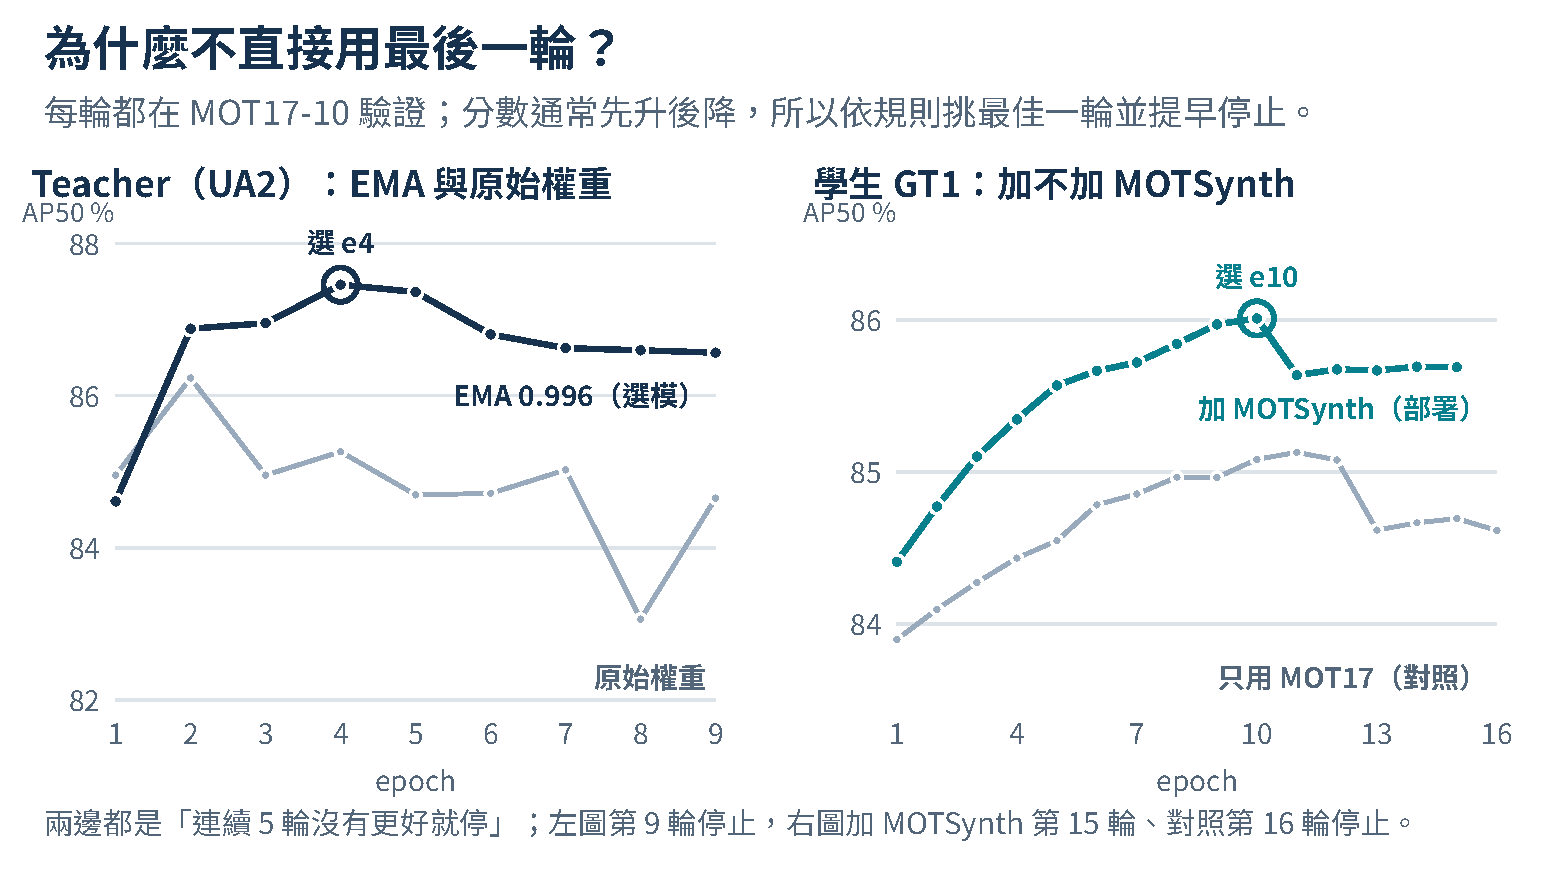
\includegraphics[width=\textwidth]{assets/train-curves.pdf}
\caption{左：Teacher 的 EMA 權重比原始權重平穩；右：學生 GT1 加入 MOTSynth 後，每一輪都高於只用 MOT17 的同預算對照。縱軸未從零開始。}
\end{figure}

\textbf{EMA 是權重的移動平均。} 每次更新後，另外保存一份「舊權重 99.6\% ＋新權重 0.4\%」的平均版，用它來驗證和選模。單一輪的權重會隨最後幾批資料晃動；平均版把這些晃動抹平。GT1 加上 EMA 後，相鄰兩輪 AP50 的平均跳動從 0.47 降到 0.15 個百分點，選到哪一輪比較不靠運氣；但最高點沒有因此變高。\cite{hrtrain}

\textbf{早停。} 連續 5 輪沒有更好就停止，省下後段注定退步的訓練時間。早停與 EMA 只是避開過度擬合，沒有消除它：每個階段最後都會退步。

\clearpage
\section{一路改了什麼，各帶來多少}
\begin{figure}[H]
\centering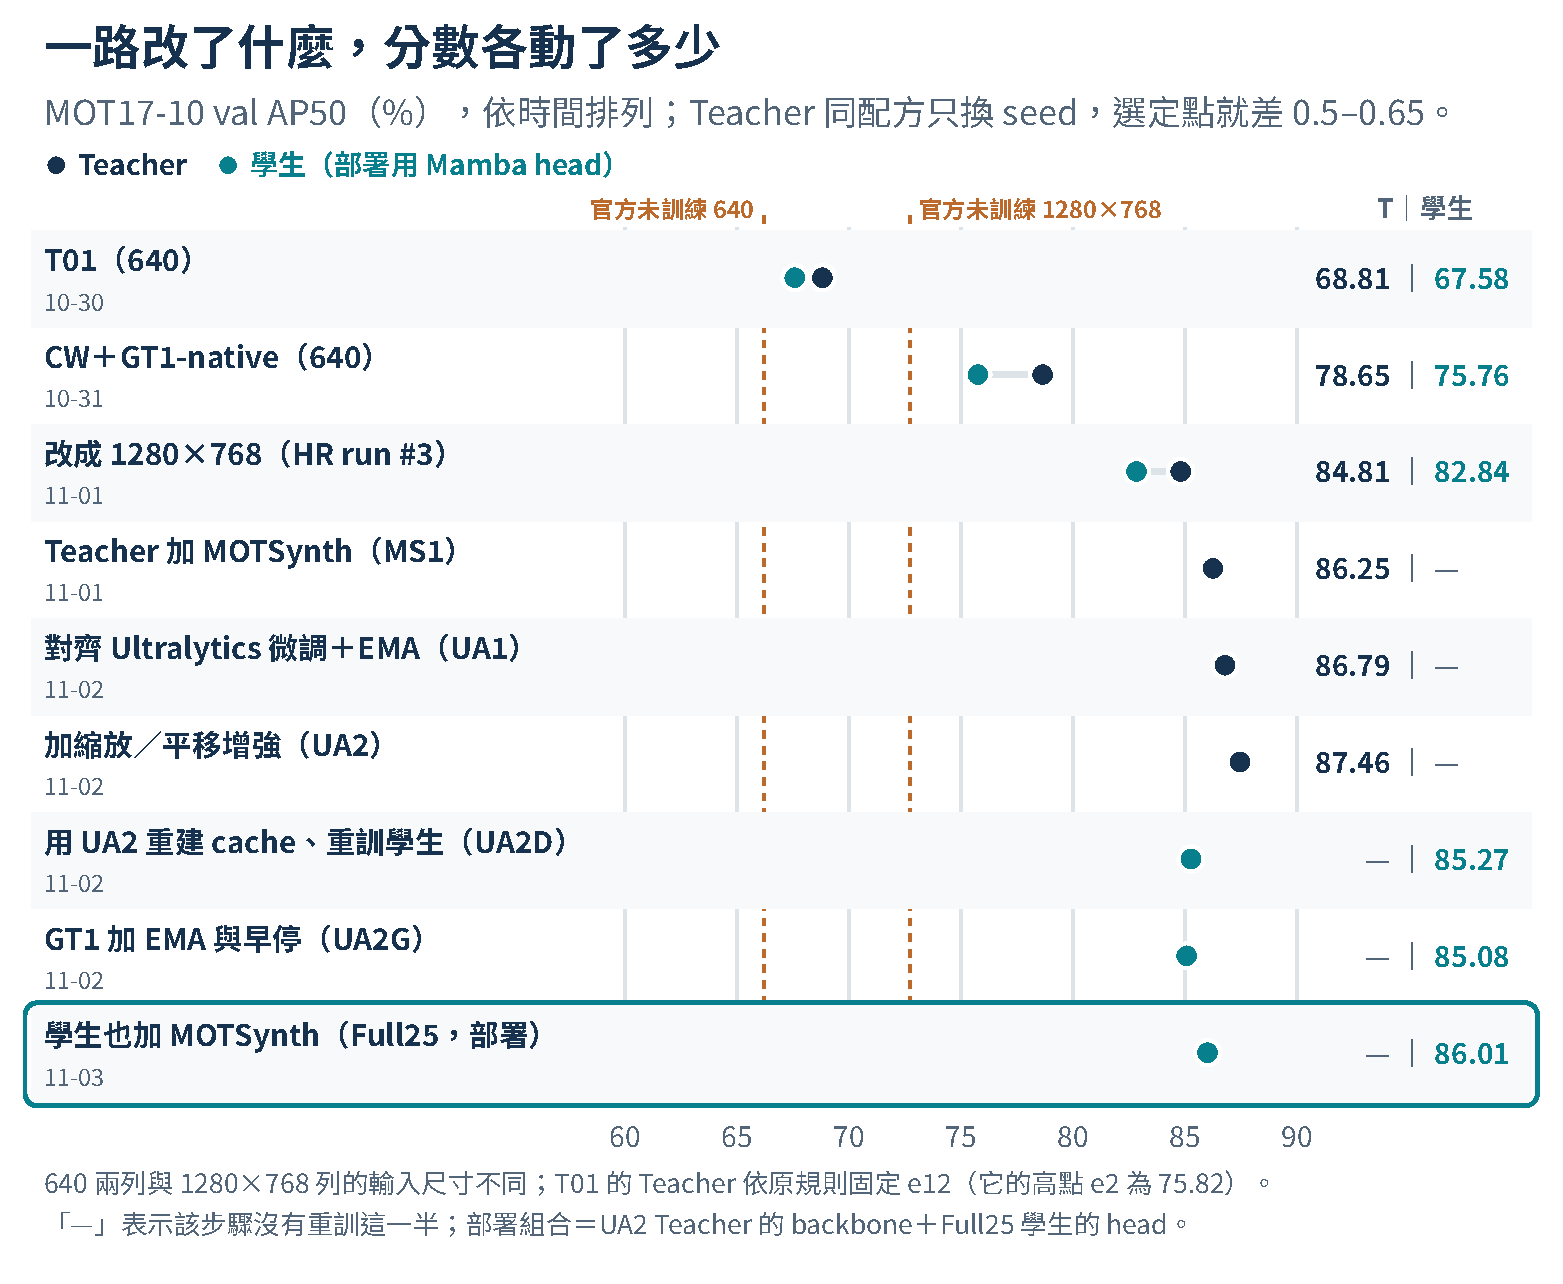
\includegraphics[width=0.9\textwidth]{assets/train-progress.pdf}
\caption{依時間排列的主要改動。每列標出 Teacher 與學生的選定點；空白代表該步沒有重訓那一半。}
\end{figure}

\textbf{效果最清楚的兩步。} 一是\textbf{改成 1280×768}：只改解析度，Teacher 與最後學生各高約 6.2 與 7.1 個百分點，主要來自小目標；最短邊 4--8 px 的召回率約加倍（GT1 19.2\%→42.3\%）。二是\textbf{換用更好的 Teacher 重訓學生}：同樣的學生配方，GT1 高 2.43 個百分點，誤檢也變少。\cite{hrtrain}

\textbf{在雜訊附近的幾步。} Teacher 同一配方只換 seed，選定點就差 0.5--0.65 個百分點。UA2 對 UA1 的 +0.67 與這個差距相當，第二個 seed 的 UA2 甚至與 UA1 幾乎相同，所以不能說增強提高了最佳點；兩個 seed 都成立的是\textbf{退步變慢、小目標整體較高}（e2--e9 平均小目標召回率高 3--4.6 個百分點）。部署的學生對同預算、只用 MOT17 的對照 AP50 +0.88，但只跑一個 seed；小目標召回率在固定 0.25 門檻時 +4.62，在相同 1,662 個誤檢下只 +2.29（附錄 B），表示部分增益來自分數分布改變。\cite{hrtrain,hrmixed}

\textbf{試過但沒有採用的。} CrowdHuman（選定點幾乎不變）、兩種外部資料合用（不勝過只加 MOTSynth）、640 版的 T3→T1 時序階段，以及 MOTSynth 從 3,056 張子集擴成完整 68,760 張候選池（+0.06，視為沒有差別；部署版本仍是完整候選池那一輪）。640 兩列的改動不只一項，也和 1280×768 列的輸入尺寸不同，不能逐列相減當成單一因素的效果。\cite{hrtrain,hrmixed,cw}

\begin{finding}
\textbf{比較穩的結論：} 解析度與 Teacher 品質是學生分數的主要來源；合成資料能延後過度擬合。\par
\textbf{還不能下結論的：} 增強、Ultralytics 配方對齊、學生端加 MOTSynth 各自讓最佳點提高多少，需要第二個 seed 才能分辨。
\end{finding}

\clearpage
\section{從訓練權重到 TensorRT engine}
訓練與匯出在 PyTorch 完成；部署端是 C++／CUDA／TensorRT，不需要 Python。中間每一步都先核對數字，才往下一步走。

\begin{figure}[H]
\centering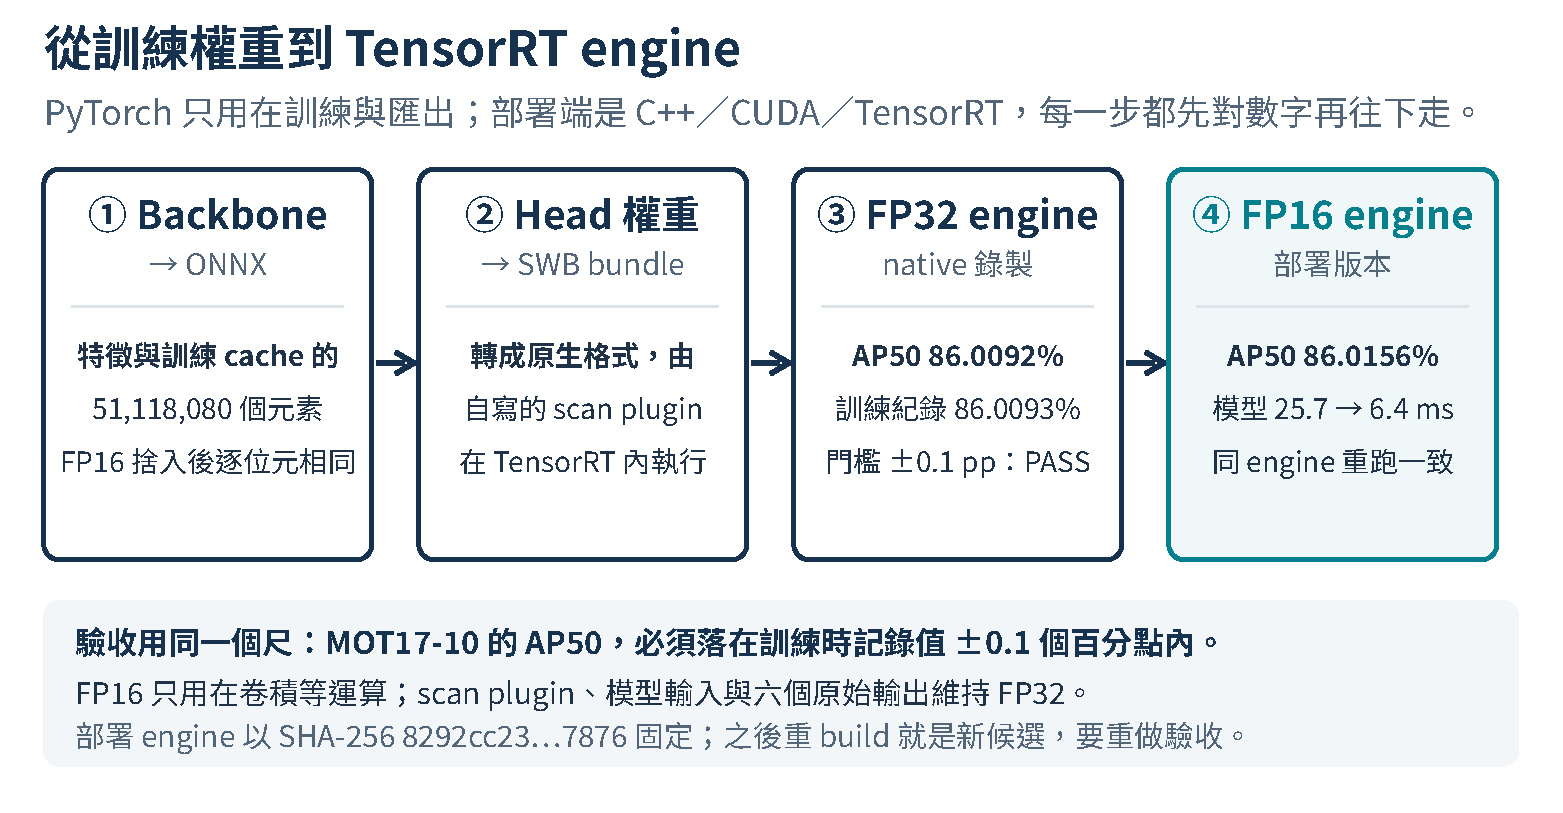
\includegraphics[width=\textwidth]{assets/train-deploy.pdf}
\caption{匯出與部署驗收。通過標準都在產生 native 結果之前固定。}
\end{figure}

\textbf{先確認匯出的是哪一份權重。} Teacher 的 checkpoint 同時存著原始權重與 EMA 權重。匯出 backbone 後，拿它算出的特徵和訓練 cache 比：EMA 權重在 FP16 捨入後與 cache 的 51,118,080 個元素完全相同，原始權重則有超過五千萬個元素不同。這證明學生訓練時看到的就是部署的 backbone。\cite{deploy}

\textbf{再用同一把尺驗收。} 原生程式錄下 MOT17-10 的偵測結果，用與訓練相同的 AP50 計算：FP32 engine 為 86.0092\%，訓練紀錄為 86.0093\%，差 0.0001 個百分點，在事先固定的 ±0.1 範圍內。\cite{deploy}

\textbf{部署改用 FP16。} FP32 時，卷積約占 GPU 時間 80\%。改成 FP16 後，模型每幀從 25.7 ms 降到 6.4 ms，AP50 為 86.0156\%，同樣在 ±0.1 範圍內；BF16 較慢、誤差約為 FP16 的 7 倍，沒有採用。自訂 scan plugin、模型輸入與六個原始輸出仍維持 FP32。部署 engine 以 SHA-256 固定，之後任何重新 build 都視為新候選，要重做同樣的驗收。\cite{deploy}

\clearpage
\section{結果怎麼看，還有哪些限制}
\textbf{最後才打開的 MOT17-02。} 選定後只評一次：AP50 為 72.91\%，比選模序列低 13.1 個百分點；前一版 640 模型（T01）在 02 為 54.40\%，落差同樣約 13 個百分點。追蹤 HOTA 由 31.6 升到 40.6，但提升全部來自偵測（DetA 23.7→40.9）；身份關聯沒有變好（AssA 42.2→40.7），IDSW 由 31 次增至 103 次。\cite{m4}

\textbf{學生沒有在選模序列上超過 Teacher。} 在 MOT17-10，學生 86.01\% 仍比 Teacher 87.46\% 低 1.45 個百分點。第一份報告中的「微調 YOLO26m」就是這個 UA2 Teacher 用它自己的 YOLO head 輸出。把三個模型接上同一套追蹤流程後，HR Mamba 在未參與訓練的 MOT20 與 MOT17-02 較高（HOTA 相對微調版 +7.74 與 +2.86），在 DanceTrack、PersonPath22 較低，平均每幀延遲多約 15--17\%。Mamba head 有沒有價值，要看資料場景，不能只看這裡的 val 分數。\cite{report1}

\textbf{這份訓練紀錄的限制}
\begin{itemize}
\item \textbf{驗證只有一段。} 所有選擇都在 MOT17-10 上做，val 分數因此偏樂觀；學生階段多為單一 seed。
\item \textbf{資料已曝光。} MOT17 七段都已在本機分析或評估過，跨資料集比較也不是盲測；MOTSynth 的 764 段 Teacher 與學生共用，不屬官方 MOTSynth 協定。
\item \textbf{不是逐位元重現。} Teacher 的中斷恢復可逐位元相同；GT1 使用非決定性 cuDNN，重跑只會在容差內一致。
\item \textbf{訓練程式在研究庫。} 本庫只保留 T01 訓練與 HR 匯出工具；HR 各階段的程式、紀錄與曲線在研究庫 \code{saccade_v1_dev} 的本機 \code{research} 分支（\code{92542386}），尚未推到遠端。大型 checkpoint 與 cache 存在 \path{~/.cache}，不進 Git。
\end{itemize}

\begin{finding}
\textbf{接下來值得回答的問題}\par
學生端加 MOTSynth 的收益換 seed 是否仍在？合成資料比例從 25\% 提到 50\% 會怎樣？能否另立一組與訓練場景完全隔離的驗證序列，讓選模不再只依賴 MOT17-10？
\end{finding}

這些是由本次整理帶出的問題；製作這份報告時沒有重新訓練、推論、計分或調參。

\appendix
\clearpage
\section{部署 lineage 的完整配方}
\small
\begin{longtable}{@{}P{2.6cm} P{12.2cm}@{}}
\toprule
項目 & 內容 \\
\midrule
\endhead
\multicolumn{2}{@{}l}{\textbf{① Teacher：UA2 seed 1（\code{HR01-UA2-20261102}）}} \\
起點 & 官方 \code{yolo26m.pt}（SHA-256 \sha{401cea9a…0745d0b7}）；gate 關閉；BatchNorm 統計值凍結；保留 80 類 head，行人為 class 0 \\
資料 & MOT17 04／05／09／11／13 與 MOTSynth 交替，每個 MOT17 批次後接一個 MOTSynth 批次；每批 4 段 clip × 2 幀＝8 張，每輪 1,016 批 \\
最佳化 & AdamW lr 1.19e-4（Ultralytics 8.4.37 auto 規則）；梯度累積到有效 batch 64；前 3 輪 warmup（lr 由 0 起、累積數 1→8）；之後線性衰減到 1\%；梯度範數上限 10；weight decay 1e-4 \\
Loss 與精度 & v8DetectionLoss（只用 one2many 分支），box／cls／dfl 權重 7.5／0.5／1.5；bf16 前向＋FP32 loss；每個時間步各自 backward \\
增強 & 水平翻轉、亮度、對比（clip 內共用）；每張影像獨立的縮放 0.5／平移 0.1（Ultralytics \code{RandomPerspective} 的縮放＋平移部分）\\
EMA 與停止 & 主 EMA 0.996／tau 25 用於選模；patience 5、最多 30 輪；9 輪後停止，選第 4 輪：AP50 87.4623\%、小目標召回率 77.8194\% \\
\midrule
\multicolumn{2}{@{}l}{\textbf{② Cache（\code{HR01-UA2D-20261102}）}} \\
內容 & Teacher 凍結、eval、ungated；batch 1 前向；存 P3（256×96×160）、P4（512×48×80）、P5（512×24×40）與 one2many 分類／框輸出 \\
精度 & 嚴格 FP32（TF32 關閉並在程序內讀回檢查）計算，FP16 儲存；每序列首末幀重算逐位元相同（train 10/10、val 2/2）\\
\midrule
\multicolumn{2}{@{}l}{\textbf{③ Distill（\code{HR01-UA2D-20261102}）}} \\
Head 結構 & d\_model 128、d\_state 16、每尺度 1 個 block、空間降採樣 4、四方向 Cross-Scan、PixelShuffle；掃描長度 960／240／60 \\
訓練 & 單幀、batch 8；MSE(分類)＋MSE(框)；AdamW 1e-3、warmup 5＋cosine 30、梯度上限 1；掃描輸出不回傳梯度（SSM 內部固定）；30 輪，選第 21 輪：81.9401\%／80.5803\% \\
\midrule
\multicolumn{2}{@{}l}{\textbf{④ GT1 mixed Full25（\code{HR01-MS-FULL25-20261103}）}} \\
起點 & ③ 第 21 輪權重；Teacher 同 ① \\
資料 & 每次更新 16 張：12 張 MOT17（讀 ② 的 cache）＋4 張 MOTSynth（68,760 張候選池，Teacher 即時算特徵）；每輪 128 次更新 \\
訓練 & B4×T4（16 張）分成四份，各自計算 TAL 偵測 loss；掃描內部一起學（learned scan）；AdamW 1e-4、warmup 5＋cosine 30、梯度上限 1 \\
EMA 與停止 & EMA 0.998／tau 25（只驗主 EMA）；patience 5；15 輪後停止，選第 10 輪：86.0093\%／75.5576\%；整個 run 用過 7,680 張不同的 MOTSynth 影像 \\
\midrule
共同 & seed 20260612；選模 \code{t01-selection/1}；每個 run root 以 manifest 綁定原始碼、外部 tree、native build、上游 checkpoint 與輸入影像雜湊，有任何變動即停止 \\
\bottomrule
\end{longtable}
\normalsize

\clearpage
\section{權重身分與完整數字}
\small
\noindent\begin{tabularx}{\textwidth}{@{}P{3.6cm} Y@{}}
\toprule
產物 & SHA-256／識別 \\
\midrule
官方起點 & \sha{401cea9ab23ad19246ff7744859816bc599f350e93c9dd30367b6f0a0745d0b7} \\
UA2 Teacher e4（EMA） & \sha{08be5abae55d26b762e262948ded7d3deb11295aa0509ee04ad3582a2c9774cd} \\
UA2D Distill e21 & \sha{8b5403b2e2a92b5682dfc9e393ee032db3ca65b54975581c170d7a3dad29ec20} \\
Full25 GT1 e10（部署 head） & \sha{53bccffe9bdbf37bdcfc81d03e95ccbd2d142d67a557ea015b76d356e4fa5f7d} \\
部署 FP16 engine & \sha{8292cc233019d08f1b1b6cfbc12f1fe1644f66f2164fd8f50a69b660a7817876}（60,753,004 bytes） \\
Run identity & UA2 \sha{ae40a790…}；UA2D \sha{d39c0e1d…}；Full25 \sha{7f0eda0b…} \\
\bottomrule
\end{tabularx}

\vspace{4mm}
\noindent\textbf{逐步改進（MOT17-10 val AP50，\%）}\par
\noindent% Generated by render_figures.py from data/milestones.csv
\begin{tabularx}{\textwidth}{@{}l P{3.6cm} Y r r@{}}
\toprule
日期 & 步驟 & 比上一列改了什麼 & Teacher & 學生 \\
\midrule
10-30 & T01（640） & 原配方正式重訓：gated teacher 固定 e12，學生 Distill→GT1→T3→T1 & 68.81 & 67.58 \\
10-31 & CW＋GT1-native（640） & Teacher 不用 gate、凍結 BN、加首輪 warmup 與輕量增強、以 val AP50 早停；GT1 讓 SSM 內部參數一起學 & 78.65 & 75.76 \\
11-01 & 改成 1280×768（HR run \#3） & 只改輸入解析度，配方不變 & 84.81 & 82.84 \\
11-01 & Teacher 加 MOTSynth（MS1） & 每個 MOT17 批次後接一個 MOTSynth 批次 & 86.25 & — \\
11-02 & 對齊 Ultralytics 微調＋EMA（UA1） & 有效 batch 64、AdamW 1.19e-4、3-epoch warmup、權重 EMA & 86.79 & — \\
11-02 & 加縮放／平移增強（UA2） & scale 0.5、translate 0.1；部署 backbone 來自這一版 & 87.46 & — \\
11-02 & 用 UA2 重建 cache、重訓學生（UA2D） & Cache／Distill／GT1 配方不變，只換 Teacher & — & 85.27 \\
11-02 & GT1 加 EMA 與早停（UA2G） & EMA 0.998、patience 5；峰值未升，選定點較穩 & — & 85.08 \\
11-03 & 學生也加 MOTSynth（Full25，部署） & 每次更新 12 張 MOT17＋4 張 MOTSynth & — & 86.01 \\
\bottomrule
\end{tabularx}


\vspace{4mm}
\noindent\begin{minipage}{\textwidth}
\textbf{學生加 MOTSynth 的同預算比較（MOT17-10）}\par
\begin{tabularx}{\textwidth}{@{}Y r r r r@{}}
\toprule
選定模型 & AP50 & 小目標 @0.25 & TP／FP @0.25 & 小目標 @同 1,662 FP \\
\midrule
只用 MOT17（對照）e11 & 85.1285 & 70.9406 & 9,016／1,662 & 70.9406 \\
＋MOTSynth 3,056 張子集 e10 & 85.9502 & 75.5420 & 9,291／1,966 & 72.9215 \\
＋MOTSynth 完整候選池 e10（部署） & 86.0093 & 75.5576 & 9,291／1,958 & 73.2335 \\
\bottomrule
\end{tabularx}
\par\vspace{2mm}
{\footnotesize\color{muted}三組同一學生起點、每輪 128 次更新、每次 16 張；對照只有 MOT17。完整曲線見 \path{data/2026-11-03-full25-epochs.csv}。}
\end{minipage}
\normalsize

\section{重跑與核對入口}
\textbf{本報告的圖表與 PDF。} 只讀 \path{data/} 內的 CSV 快照（取自研究庫 \code{92542386}，雜湊見 \path{figures.json}），不啟動模型、訓練或計分。於專案根目錄執行：
{\small
\begin{verbatim}
python3 -B docs/reports/latex/training/render_figures.py
make -C docs/reports/latex/training
\end{verbatim}
}

\textbf{HR 訓練（研究庫 \code{saccade_v1_dev}）。} 每個 run 先跑 smoke root；正式 root 中斷後加 \code{--resume}，從最後一個已提交的 epoch 接續。Teacher／Cache／Distill／GT1 的配方在 \path{training/hr/recipe.json} 的 variant（UA2、UA2D）。
{\small
\begin{verbatim}
training/hr/hr_pipeline.py      prepare|run|status    --root build-hr/<name>
training/hr_mixed/runner.py     prepare|launch|status --root build-hr-mixed/<name>
\end{verbatim}
}

\textbf{匯出與部署（本庫）。} \path{training/hr_deploy/README.md} 列出 head 權重轉換、backbone ONNX 匯出與驗證、參考輸入與 manifest 的完整指令；驗收步驟見 \path{docs/TRACKING.md} §15--§16。Engine 由下列指令產生：
{\small
\begin{verbatim}
model_trt build --precision fp16 --profile hr-1280x768 ...
\end{verbatim}
}

\textbf{較早的 640 訓練（本庫）。} \path{training/t01/} 與 \path{docs/T01_TRAINING.md}，含資料切分 manifest、前處理與精度契約。

\clearpage
\begin{thebibliography}{9}
\footnotesize
\setlength{\itemsep}{0.3em}
\bibitem{t01} T01 訓練規格與執行紀錄：\path{docs/T01_TRAINING.md} §1--§8；資料切分 \path{manifests/t01/split.json}；程式 \path{training/t01/}。
\bibitem{hrtrain} HR 訓練（1280×768、Teacher 資料來源、UA1／UA2／UA2S2、UA2D、UA2G）：研究庫 \code{92542386} 的 \path{docs/HR_TRAINING.md} §1--§16、\path{training/hr/}、\path{evidence/hr/2026-11-02/}。
\bibitem{hrmixed} 學生加 MOTSynth（control／subset25／Full25）：研究庫 \code{92542386} 的 \path{docs/HR_MOTSYNTH_STUDENT.md}、\path{training/hr_mixed/}、\path{evidence/hr/2026-11-03/full25/REPORT.md}。
\bibitem{cw} 640 版 CW Teacher 與下游：研究庫 \path{docs/TEACHER_CW_EXPERIMENT.md}、\path{docs/CW_PIPELINE_TRAINING.md}、\path{docs/GT1_NATIVE_RESULTS.md}。
\bibitem{deploy} HR 部署與 FP16：\path{training/hr_deploy/README.md}；\path{docs/TRACKING.md} §15--§16；\path{evidence/precision/2026-11-03-formal/}。
\bibitem{m4} MOT17-02 最終評估：\path{docs/TRACKING.md} §17.5；\path{evidence/m4/2026-11-03-formal-cad5298/REPORT.md}。
\bibitem{report1} 第一輪圖解報告：\path{docs/reports/latex/report1/report.pdf}；訓練來源對照 \path{evidence/model-comparison/2026-11-11-yolo26m-primary156/bundle/training-provenance.json}。
\end{thebibliography}
\end{document}
